%%%%%%%%%%%%%%%%%%%%%%% file template.tex %%%%%%%%%%%%%%%%%%%%%%%%%
%
% This is a general template file for the LaTeX package SVJour3
% for Springer journals.          Springer Heidelberg 2010/09/16
%
% Copy it to a new file with a new name and use it as the basis
% for your article. Delete % signs as needed.
%
% This template includes a few options for different layouts and
% content for various journals. Please consult a previous issue of
% your journal as needed.
%
%%%%%%%%%%%%%%%%%%%%%%%%%%%%%%%%%%%%%%%%%%%%%%%%%%%%%%%%%%%%%%%%%%%
%
\RequirePackage{fix-cm}
%
%\documentclass{svjour3}                     % onecolumn (standard format)
%\documentclass[smallcondensed]{svjour3}     % onecolumn (ditto)
\documentclass[smallextended]{svjour3}       % onecolumn (second format)
%\documentclass[twocolumn]{svjour3}          % twocolumn
%
\smartqed  % flush right qed marks, e.g. at end of proof
%
\usepackage{graphicx}
\usepackage[numbers]{natbib}
\usepackage{bussproofs}
\usepackage{tikz}
\usepackage{amssymb}
\usepackage{amsmath}
\usepackage[all,cmtip]{xy}
\usetikzlibrary{positioning, automata}
\usetikzlibrary{decorations.pathmorphing}

\tikzset{snake it/.style={decorate, decoration=snake}}

\usepackage[T1]{fontenc}
\DeclareFontFamily{T1}{calligra}{}
\DeclareFontShape{T1}{calligra}{m}{n}{<->s*[1.44]callig15}{}
\DeclareMathAlphabet\mathzapf       {T1}{pzc} {mb} {it}


%
% \usepackage{mathptmx}      % use Times fonts if available on your TeX system
%
% insert here the call for the packages your document requires
%\usepackage{latexsym}
% etc.
%
% please place your own definitions here and don't use \def but
% \newcommand{}{}
%
% Insert the name of "your journal" with
% \journalname{myjournal}
%
\begin{document}


\title{Parallel Complexity of CFL-Reachability Problem: Tractable Cases%\thanks{Grants or other notes
%about the article that should go on the front page should be
%placed here. General acknowledgments should be placed at the end of the article.}
}
%\subtitle{Do you have a subtitle?\\ If so, write it here}

%\titlerunning{Short form of title}        % if too long for running head

\author{Ekaterina Shemetova         \and
         Alexander Okhotin
         \and Semyon Grigorev %etc.
}

%\authorrunning{Short form of author list} % if too long for running head

\institute{E. Shemetova \at
             St. Petersburg Academic University, ul. Khlopina, 8, Saint Petersburg 194021, Russia, and \\ JetBrains Research \\
              \email{katyacyfra@gmail.com}           %  \\
%             \emph{Present address:} of F. Author  %  if needed
           \and
           A. Okhotin \at
              St. Petersburg State University, 7/9 Universitetskaya nab., Saint Petersburg 199034, Russia, 
           \and
           S. Grigorev \at
              St. Petersburg State University, 7/9 Universitetskaya nab., Saint Petersburg 199034, Russia, 
and  JetBrains Research  \\
              \email{s.v.grigoriev@spbu.ru}    
}

\date{Received: date / Accepted: date}
% The correct dates will be entered by the editor


\maketitle

\begin{abstract}
Whereas it has been shown that  context-free language (CFL) reachability problem is P-complete, there are some subclasses of context-free languages, for which CFL-reachability lies in NC complexity class. We present two common classes which generalize known examples of such tractable subclasses: bounded-oscillation languages and context-free languages with a poly-slender storage languages. Polynomiality of the rational indices of languages in these classes is proved. Polynomial time algorithm for deciding whether a given PDA has poly-slender storage language is given. Closure properties of tractable subclasses in terms of polynomial rational index are investigated. 




\keywords{CFL-reachability \and parallel complexity \and graphs \and regular languages \and context-free languages \and context-free path queries}
% \PACS{PACS code1 \and PACS code2 \and more}
% \subclass{MSC code1 \and MSC code2 \and more}
\end{abstract}



\section{Introduction}
\label{intro}
The context-free language (CFL) reachability problem for a context-free grammar $G$ and directed edge-labelled graph $D$ consists of determining for pairs of nodes  $v$ and $u$ whether $v$ can reach $u$ via a path labelled by a string in $L(G)$.  That is, CFL-reachability is a kind of graph reachability problem with path constraints given by context-free languages. It is an important problem underlying some fundamential static code analysis like data flow analysis and program slicing \cite{RepsBasic}, alias analysis \cite*{Chatterjee, alias}, points-to analysis \cite{Incremental} and other \cite*{Cai, android, typeflow}, and graph database query evaluation \cite*{Azimov, GrigorevRagozina, HellingsCFPQ, RDF}.


Unlike context-free language recognition, which is in NC (when context-free grammar is fixed), CFL-reachability is P-complete \cite*{ RepSeq, Yannakakis}. Practically, it means that there is no efficient parallel algorithm for solving this problem (unless P $\neq$ NC). 


While problem is not parallelizable in general, it is useful to develop more efficient parallel solutions for specific subclasses of context-free languages. For example, there are context-free languages which admit more efficient parallel algorithms in comparision with the general case of context-free recognition \cite*{IBARRA, IBARRA2, Okhotin2014ComplexityOI}.  The same holds for CFL-reachability problem: there are some examples of context-free languages, for which CFL-reachability problem lies in NL complexity class (for example, linear and one-counter languages) \cite*{LabelledGraphs, LReach, Regularrealizability}. 


CFL-reachability problem has long been known to be P-complete \cite{PCompl}. A parallel complexity of this problem is studied by both static code analysis \cite*{RepSeq, RepsBasic} and database communities \cite*{ChainQ, Ullman, Yannakakis}. First investigations of such type were made in terms of Datalog queries, because some classes of Datalog queries (logic programs
without function symbols) can be represented via context-free grammars, while database can be considered as a graph. Important decidability result is obtained in \cite{Vardi}: given a context-free grammar (query) and an arbitrary graph (database), it is undecidable whether CFL-reachability problem for them is in NC or P-complete. However, Ulman and Van Gelder in \cite{Ullman} introduce a notion of a  \textit{polynomial fringe property} and show that a context-free grammars having this property are in NC. A context-free grammar $G$ has the \textit{polynomial fringe property} if and only if there is a polynomial $p$ such that, for each regular language $R$ recognized by an automaton with $n$ states, $L(G) \cap R$ is either empty or contains a word shorter than $p(n)$. It is undecidable whether a context-free grammar has the polynomial fringe property. Important results from \cite{Ullman} can be reinterpreted in terms of CFL-reachability as follows: 
\begin{enumerate}
\item CFL-reachability for linear languages and piecewise linear languages, and for arbitrary graphs is in NC, because corresponding grammars have the polynomial fringe property
\item The same holds for $D_1$ (the Dyck language on one kind of parentheses) and its GSM-mappings (one-counter languages)
\item CFL-reachability for $D_2$ (the Dyck language on two kinds of parentheses) is P-complete.
\end{enumerate}
The third result is important because any context-free language can be represented via a regular language and $D_2$, which are combined by means of an intersection and a homomorphism, so it is the direct consequence of P-competeness of CLF-reachability problem in general. Also, using the fact that $D_2$ is included in many interesting subclasses of context-free languages, such as visibly pushdown languages \cite{Okhotin2014ComplexityOI}, simple deterministic languages (defined by LL(1) grammars in Greibach normal form), we can state that CFL-reachability for these languages is P-complete. Afrati et al. \cite{ChainQ} investigate parallel complexity of Datalog simple chain queries and presents the Polynomial Stack Lemma which will be discussed in detail in Section~\ref{sec:poly}. 


The definition of polynomial fringe property coincides with the notion of a so called \textit{rational index}: for a context-free language $L(G)$ having the polynomial rational index is the same as for $G$ to have the polynomial fringe property. More precisely, rational index $\rho_L(n)$ is a function, which denotes the maximum length of the shortest word in $L(G) \cap R$, for arbitrary $R$ recognized by an $n$-state automaton. The notion of rational index was introduced in \cite{RatBasic} as a complexity measure for context-free languages and was investigated independently from the polynomial fringe property.  In particular, it has been proved that the rational index of $D_1$ is in $O( n^2)$ \cite{Dyck1}. 
Another important result concerns the rational index of languages, which generate all context-free languages (an example of such language is $D_2$). It states that the rational index of such languages is of the order $exp(\Theta(n^2/\ln n))$ \cite{CFRat} and, hence, this is the upper bound on the value of rational index for every context-free language. An example of a non-generating language with exponential rational index is given in \cite{Regularrealizability}. Also it has been shown that for every algebraic number $\gamma $ the language with the rational index in $\Theta (n^\gamma )$ exists \cite{GreibRat}. 


The CFL-reachability problem is the same as the intersection non-emptiness problem for a context-free language (pushdown automaton) and a regular language (finite automaton), because a labelled graph is a special kind of a nondeterministic finite automata. Complexity of this problem is studied by Ganardi et al. \cite{ ganardi2016circuit} ,  Swernofsky et al. \cite{Intersection}, Vyalyi \cite{VyalyiRR}.


Computational complexity of the language reachability for different variants of languages (regular, context-free, context-sensitive) and graphs (acyclic graphs, trees, grid graphs) is discussed in detail by Barret et al. \cite{Barrett}, Holzer et al.\cite{LabelledGraphs}, Komarath et al. \cite{LReach}. 


\begin{figure}
\centering
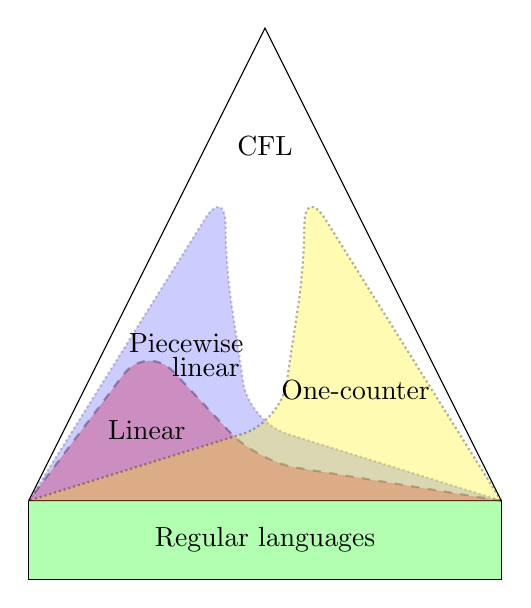
\begin{tikzpicture}
\draw[fill=green, opacity=0.3](0,1) -- (0,0) -- (6,0) --  (6,1);
\draw(0,1) -- (0,0) -- (6,0) --  (6,1);
\draw(0,1) -- (6,1) -- (3, 7) -- (0,1) ;
%\draw[thick, dashed, rounded corners=5mm, fill=yellow, opacity=0.3] (0,1) -- (3.1, 1.5) -- (4.5, 3) -- (6,1);
\draw[thick, dashed, rounded corners=5mm, fill=red, opacity=0.3] (6,1) -- (2.9, 1.5) -- (1.5, 3) -- (0,1);
\draw[thick, densely dotted, rounded corners=5mm, fill=blue, opacity=0.2](0,1) -- (2.5, 5) -- (2.5,4)-- (2.8, 2) -- (6,1);
\draw[thick, densely dotted, rounded corners=5mm , fill=yellow, opacity=0.3](6,1) -- (3.5, 5) -- (3.5,4)-- (3.2, 2) -- (0,1);
\node (reg) at (3, 0.5) {Regular languages}; 
\node (cfl) at (3, 5.5) {CFL}; 
\node (lin) at (1.5, 1.9) {Linear}; 
\node (one) at (4.15, 2.4) {One-counter}; 
\node (linsc) at (2, 3) {Piecewise};
\node (linpsc) at (2.25, 2.7)  {linear}; 
\end{tikzpicture}
\caption{The hierarchy of languages, for which CFL-reachability problem is in NC.}
\label{hierarchy}      
\end{figure}
Our focus is on investigating the parallel complexity of CFL-reachability. Especially we are interested in generalization of ``easy'' subclasses and discovering new examples of context-free languages, for which CFL-reachability is in NC. Effective subclasses can be useful in practice, because the general problem is not tractable \cite{ExperimentalCFPQ}. For example, in case of graph databases it is important to know the complexity of a given context-free path query. Also it is natural to ask which properties of subclasses imply parallel effectiveness. Why some languages have polynomial rational indices? What is the difference between them and other subclasses of context-free languages?


The hierarchy of subfamilies of context-free languages, for which the CFL-reachability problem is in NC, is presented in Figure~\ref{hierarchy}. Linear (and piecewise linear) languages and one-counter languages are uncomparable families of context-free languages, but both have polynomial rational indices (polynomial fringe property). These subfamilies have one thing in common: both are defind by strong restrictions on the stack in a pushdown automaton. Our main idea is to generalize known tractable classes by investigating the restrictions on the PDA store.

\textbf{Our contributions.} Our results can be summarized as follows:
\begin{itemize}
\item We show that the CFL-reachability problem for bounded-oscillation languages of Ganty and Valput \cite{BoundOsc}, is in NC (see Section \ref{sec:osc}). This class generalizes the case of linear languages. 
\item In Section \ref{sec:poly} we introduce a new subclass of context-free languages --- context-free languages with a poly-slender pushdown store languages. These languages are the natural generalization of one-counter languages, and the CFL-reachability problem for them is in NC. Also we show that deciding poly-slenderness of a pushdown store language is in PSPACE.  
\item Closure properties of the languages with polynomial rational indices are investigated in Section \ref{sec:closure}, particularly it is shown that the family of languages with polynomial rational indices is a full AFL.
\end{itemize}
\section{Preliminaries} \label{section_preliminaries}
In this section, we introduce the basic notions used throughout the paper.

Let $\Sigma$ be a finite set of edge labels. Define an \textit{edge-labeled directed graph} as a tuple $D = (V, E)$ with $V$ is a set of nodes and $E \subseteq V \times \Sigma \times V$ is a directed edge-relation.  For a path $\pi$ in a graph $D$ we denote $l(\pi)$ --- the unique word obtained by concatenating the labels of the edges along the path $\pi$. Also, we write $n \pi m$ to indicate that a path $\pi$ starts at node $n \in V$ and ends at node $m \in V$.

According to Hellings~\cite{hellingsRelational}, we deviate from the usual definition of a context-free grammar in \textit{Chomsky Normal Form}~\cite{chomsky} by not including a special start non-terminal, which will be specified in the queries to the graph. Since every context-free grammar can be transformed into an equivalent one in Chomsky Normal Form and checking that an empty string is in the language is trivial, then it is sufficient to only consider grammars of the following type. A \textit{context-free grammar} is 3-tuple $G = (N, \Sigma, P)$ where $N$ is a finite set of non-terminals, $\Sigma$ is a finite set of terminals, and $P$ is a finite set of productions of the following forms:

\begin{itemize}
    \item $A \rightarrow B C$, for $A,B,C \in N$,
    \item $A \rightarrow x$, for $A \in N$ and $x \in \Sigma$.   
\end{itemize}

Note that we omit the rules of the form $A \rightarrow \varepsilon$, where $\varepsilon$ denotes an empty string. This does not limit the applicability of further algorithms because checking that an empty string belongs to the context-free language in Chomsky normal form is trivial and only the empty paths $m \pi m$ correspond to an empty string $\varepsilon$.

We use the conventional notation $A \xrightarrow{*} w$ to denote that the string $w \in \Sigma^*$ can be derived from a non-terminal $A$ by some sequence of applying the production rules from $P$. The \textit{language} of a grammar $G = (N,\Sigma,P)$ with respect to a start non-terminal $S \in N$ is defined by $L(G_S) = \{w \in \Sigma^*~|~S \xrightarrow{*} w\}$.

For a given graph $D = (V, E)$ and a context-free grammar $G = (N, \Sigma, P)$, we define \textit{context-free relations} $R_A \subseteq V \times V$, for every $A \in N$, such that $R_A = \{(n,m)~|~\exists n \pi m~(l(\pi) \in L(G_A))\}$.

We define a binary operation on arbitrary subsets $N_1 , N_2$ of $N$ with respect to a context-free grammar $G = (N, \Sigma, P)$ as $N_1 \cdot N_2 = \{A~|~\exists B \in N_1, \exists C \in N_2 \text{ such that }(A \rightarrow B C) \in P\}.$

Using this binary operation as a multiplication on arbitrary subsets of $N$ and union of sets as an addition, we can define a \textit{matrix multiplication}, $a \cdot b = c$, where $a$ and $b$ are matrices of the suitable size that have subsets of $N$ as elements, as $c_{i,j} = \bigcup^{n}_{k=1}{a_{i,k} \cdot b_{k,j}}$.

We define the \textit{transitive closure} of a square matrix $a$ as $a^+ = a^{(1)} \cup a^{(2)} \cup \cdots$ where $a^{(i)} = a^{(i-1)} \cup (a^{(i-1)} \cdot a^{(i-1)})$, $i \ge 2$ and $a^{(1)} = a$.
\section{Bounded-oscillation languages}
\label{sec:osc}
Bounded-oscillation languages were introduced by Ganty and Valput \cite{BoundOsc}. Just like one-counter and linear languages, it is defined by restriction on the pushdown automata. This restriction is based on the notion of \textit{oscillation}, a special measure of how the stack height varies over time. Oscillation is defined using a hierarchy of \textit{harmonics}. Let $\bar{a}$ be a \textit{push}-move and $a$ be a \textit{pop}-move. Then a PDA run can be recursively described by well-nested subsequence of $\bar{a}$-s and $a$-s as follows:
\begin{itemize}
\item  order 1 harmonic $h_1$ is $\bar{a}a\bar{a}a$ (\textit{push pop push pop})
\item  harmonic $h_2$ is $\bar{a}$ <order 1 harmonic> $a\bar{a}$ <order 1 harmonic> $a$
\item  $h_{(i+1)}$ harmonic is $\bar{a}h_ia\bar{a}h_ia$.
\end{itemize}
\begin{figure}
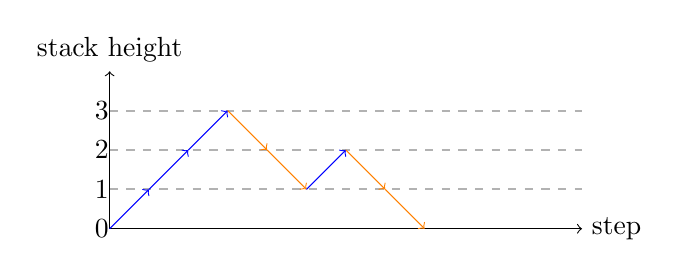
\begin{tikzpicture}
    \draw[thick, dashed, opacity=0.3] (0,0.5) -- (6,0.5);
     \draw[thick, dashed, opacity=0.3] (0,1) -- (6,1);
      \draw[thick, dashed, opacity=0.3] (0,1.5) -- (6,1.5);
      \draw[->] (0,0) -- (6,0) node[right] {step};
      \draw[->] (0,0) -- (0,2) node[above] {stack height};
     \draw[->, blue] (0,0) -- (0.5,0.5);
      \draw[->, blue] (0.5,0.5) -- (1,1);
      \draw[->, blue] (1,1) -- (1.5,1.5);
       \draw[->, orange] (1.5,1.5) -- (2,1);
    \draw[->, orange] (2,1) -- (2.5,0.5);
    \draw[->, blue] (2.5,0.5) -- (3,1);
    \draw[->, orange] (3,1) -- (3.5,0.5);
 \draw[->, orange] (3.5,0.5) -- (4,0);
\node (null) at (-0.1, 0) {0}; 
\node (one) at (-0.1, 0.5) {1}; 
\node (two) at (-0.1, 1) {2}; 
\node (three) at (-0.1, 1.5) {3}; 
    \end{tikzpicture}
\caption{Stack heights during the run of PDA.}
\label{oscb}
\end{figure}


PDA run $r$ is \textit{k-oscillating} if the harmonic of order $k$ is the greatest harmonic that is contained in $r$. \textit{Bounded-oscillation languages} are languages accepted by pushdown automata restricted to k-oscillating runs. It is important that the problem whether a given CFL is a bounded-oscillation language is undecidable \cite{BoundOsc}.
\begin{example}
Consider Figure \ref{oscb}. It shows how the stack height changes during the run of a PDA. Corresponding well-nested word is $\bar{a}\bar{a}\bar{a}aa\bar{a}aa$. The greatest harmonic in this word is order 1 harmonic (moves forming harmonic are marked in bold): $\bar{a}\bar{a}\mathbf{\bar{a}a}a\mathbf{\bar{a}a}a$, therefore oscillation of the run is 1.
\end{example}


Oscillation of the run is closely related with the $dimension$ of the corresponding parse tree. For each node $v$ in a tree $T$ a dimension $dim(v)$ is inductively defined as follows:
\begin{itemize}
\item If $v$ is a leaf, then $dim(v)$ = 0
\item If $v$ is an internal node with $k$ children $v_1, v_2, ..., v_k$ for $k \ge 1$, then 
$$
dim(v) = 
 \begin{cases}
   \max_{i \in \{1...k\}}dim(v_i) &\text{if there is a unique maximum}\\
   \max_{i \in \{1...k\}}dim(v_i)+1 &\text{otherwise}
 \end{cases}
$$
\end{itemize}


Dimension of a parse tree $T$ $dim(T)$ is a dimension of it's root.  It is observable from the definition that dimension of a tree $T$ is the height of the largest perfect binary tree, which can be obtained from $T$ by contracting edges and accordingly identifying vertices. A tree with dimension $dim(T) = 2$ is illustrated in Figure \ref{oscbtree}.


It is known that the dimension of parse trees and the oscillation defined on PDA runs are in linear relationship.

\begin{lemma}[\cite{BoundOsc}]
\label{boscdim}
Let a grammar $G = (\Sigma, N, P, S)$ be in Chomsky normal form and let $T$ be a parse tree of $G$. Then $osc(T) - 1 \le dim(T) \le 2osc(T)$.
\end{lemma}

Before we consider the value of the rational index for $k$-bounded-oscillation languages, we need to prove the following.
\begin{figure}
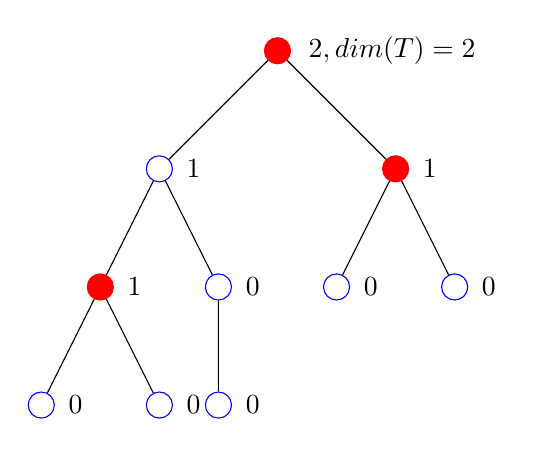
\begin{tikzpicture}[
level 1/.style={sibling distance=3cm},
level 2/.style={sibling distance=1.5cm}]
%\tikzstyle{every node}=[circle,draw]

\node[circle,draw] (Root) [ fill=red, red] {}
    child {
    node[circle,draw, blue] (l) {} 
    child { node[circle,draw, fill=red, red](ll) {}
            child { node[circle,draw, blue] (p) {} }
            child { node[circle,draw, blue] (pl) {} }
             }
    child { node[circle,draw, blue](lr) {} 
          child { node[circle,draw, blue] (plr) {} }
      }
}
child {
    node[circle,draw,  fill=red, red] (r) {}
    child { node[circle,draw, blue] (rl) {}} 
    child { node[circle,draw, blue] (rr) {} }
};
\node  [right=0.05cm of p] {0};
\node  [right=0.1cm of Root] {$2, dim(T)=2$};
\node  [right=0.05cm of l] {1};
\node  [right=0.05cm of r] {1};
\node  [right=0.05cm of ll] {1};
\node  [right=0.05cm of lr] {0};
\node  [right=0.05cm of pl] {0};
\node  [right=0.05cm of plr] {0};
\node  [right=0.05cm of rl] {0};
\node  [right=0.05cm of rr] {0};
\end{tikzpicture}
\caption{A tree $T$ with $dim(T)=2$. Nodes having children without unique maximum are filled.}
\label{oscbtree}            
\end{figure}
\begin{lemma}
\label{lem:treeheight}
Let  $G = (\Sigma, N, P)$ be a context-free grammar,  $D=(V, E, \Sigma)$ be a directed labelled graph with $n$ nodes. Let $w$ be the shortest string in $L(G)\cap L(D)$. Then a height of a parse tree for $w$ does not exceed $|N|n^2$.
\end{lemma}

\begin{proof}
 Assume that the parse tree for $w$ has a height of more than $|N|n^2$. There are $|N|n^2$ unique labels $(A, i, j)$ for nodes of the parse tree, so according to the pigeonhole principle, the parse tree for $w$ contains at least one subtree $T$ with label $(A, i, j)$ at the root, which has a subtree $T'$ with the same label. Then we can change $T$ with $T'$ and get a new string $w'$ which is shorter than $w$. But $w$ is the shortest, then we have a contradiction.

\end{proof}
From Lemma \ref{lem:treeheight} we have that rational index of linear languages is in $O(n^2)$. 
\begin{lemma}
\label{oscbnddim}
Let $G$ be a grammar $G = (\Sigma, N, P, S)$ in Chomsky normal form, such that every parse tree $T$ has $dim(T) \le d$, where $d$ is some constant. Let $D=(V, E, \Sigma)$ be a directed labelled graph with $n$ nodes. Then $\rho_{L(G)}$ is in $O({(|N|n^2)}^d)$.
\end{lemma}
\begin{proof}
Proof by induction on dimension $dim(T)$.
\\
\textbf{Basis.} $dim = 1$.
\\
Consider the worst-case tree $T$ with the dimension $dim(T) = 1$. The root of the tree has the same dimension and has two children (because the grammar in Chomsky normal form). There are two cases:  first, when both of child nodes have dimension equal to 0, then the tree has only two leaves and second, when one of children has a dimension 1, and the second child has a dimension equal to 0. For the second case we can recursively construct a tree of maximum height $|N|n^2$ (Lemma \ref{lem:treeheight}). Every internal node of such tree has two children, one of which has dimension equal to 0 and therefore has only one leaf. This tree is exactly the worst-case tree for linear grammar in Chomsky normal form, so the number of leaves in such tree is $O(h) = O(|N|n^2)$, where $h$ is the height of the tree. 
\\
\textbf{Inductive step.} $dim = d + 1$.
\\
Assume that $\rho_{L(G)}$ is no more than $O(h^{d})$ for every $d$, where $h$ is the height of the tree. We have two cases for the root node with dimension equal to $d+1$: 1) both of children have a dimension equal to $d$, then by proposition the tree of heght $h$ has no more than $O(h^{d})$ leaves; 2) one of children has a dimension $d + 1$, and the second child $v$ has a dimension $dim(v) \le d$. Again, a tree of maximum height with the maximum number of leaves can be constructed recursively:  each node of such tree has two children $u$ and $v$ with dimension $d+1$ and $d$ respectively (the more value of dimension of the node, the more leaves in the corresponding tree). By proposition we have no more than $(h-1)^d + (h-2)^d + (h-3)^d + ... + 1 = O(h^{d+1})$ leaves, so proposition holds for $dim = d+1$. Finally, we have $\rho_{L(G)}$ is no more than $O(h^{d}) = O({(|N|n^2)}^d)$ for every $d$.
\end{proof}
Combining Lemma \ref{boscdim} and Lemma \ref{oscbnddim}, we can deduce the following.
\begin{theorem}
\label{oscbndosc}
Let $L$ be a $k$-bounded-oscillation language with grammar $G = (\Sigma, N, P, S)$ in Chomsky normal form and $D=(V, E, \Sigma)$ be a directed labelled graph with $n$ nodes. Then $\rho_{L(G)}$ is in $O((|N|n^2)^{k/2})$.
\end{theorem}

As we can see from the proof above, the family of linear languages is included in the family of bounded-oscillation languages. The reason is that the family of bounded-oscillation languages generalizes the family of languages accepted by finite-turn pushdown automata \cite{BoundOsc}. It is interesting that for arbitrary CFL, particularly for $D_2$, the value of osciillation is not constant-bounded: it depends on the length of input and does not exeed $O(\log n)$ for the input of length $n$ \cite*{Gundermann, Wechsung}. However, for some previously studied subclasses of context-free languages,  oscillation is bounded by a constant.

\begin{example}[Superlinear languages \cite{superlinear}.]
\\
A context-free grammar $G = (\Sigma, N, P, S)$ is \textit{superlinear} if all productions of $P$ satisfy these conditions:
\begin{enumerate}
\item there is a subset $N_L \subseteq N$ such that every $A \in N_L$ has only linear productions $A\rightarrow aB$ or $A\rightarrow Ba$, where $B \in N_L$ and $a \in \Sigma$.
\item if $A \in N \setminus N_L$, then $A$ can have non-linear productions of the form $A \rightarrow BC$ where $B\in N_L$ and $C \in N$, or linear productions of the form $A\rightarrow \alpha B$ | $B \alpha$ | $\alpha$ for $B \in N_L$, $\alpha \in \Sigma^*$.
\end{enumerate}
From the grammar $G$ it is observable that its parse trees have dimension at most 2. From 
Lemma~\ref{oscbnddim}, if dimensions of all parse trees are bounded by some $k$ then the rational index of such language is polynomial, so CFL-reachability problem for superlinear languages and an arbitrary graph is in NC. 
\end{example}
\begin{figure}
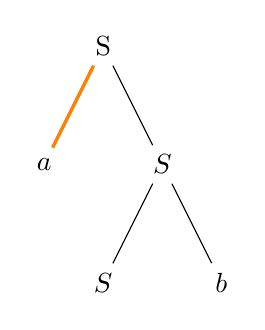
\begin{tikzpicture}
\node{S}
 child [very thick, orange] {node [black] {$a$} }
 child {node {$S$}
      child {node {$S$}}
     child {node {$b$}}
         };
\end{tikzpicture}
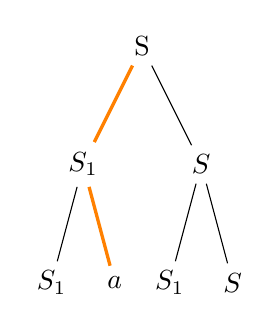
\begin{tikzpicture}[level 2/.style={sibling distance=8mm}]
\node{S} 
child [very thick, orange]  {node [black]  {$S_1$}
     child  [thin, black] {node {$S_1$}}
     child {node [black] {$a$}}
}
child  {node {$S$}
    child {node {$S_1$}}
    child {node {$S$}}
};
\end{tikzpicture}
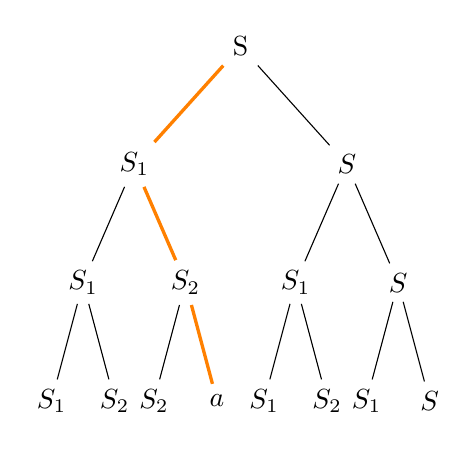
\begin{tikzpicture}[level 1/.style={sibling distance=27mm}, level 2/.style={sibling distance=13mm},  level 3/.style={sibling distance=8mm}]
\node{S} 
child [very thick, orange]  {node [black]   {$S_1$}
     child  [thin, black] {node {$S_1$} 
             child {node {$S_1$}}
             child {node {$S_2$}
                }}
     child {node [black]   {$S_2$}
                 child [thin, black] {node {$S_2$}}
                child {node [black]   {$a$}}
               }
}
child  {node {$S$}
    child {node {$S_1$}
                       child {node {$S_1$}}
             child {node {$S_2$}}
}
    child {node {$S$}
             child {node {$S_1$}}
             child {node {$S$}
                }}
};
\end{tikzpicture}
\caption{A parse trees and critical paths for piecewise linear grammars in the Chomsky normal form for $|N| = 1, 2, 3$.}
\label{crit}      
\end{figure}
\begin{example}[Piecewise linear languages.]
\\
The family of piecewise linear queries is known to be a large class of Datalog queries which have polynomial fringe property \cite{Ullman}. Those queries can be described via piecewise linear grammars. A grammar $G = (\Sigma, N, P, S)$ is \textit{piecewise linear} if every nonterminal symbol $A \in N$ generates a derivation with at most one $A$ by any sequence of applying the production rules. A piecewise linear language is a language generated by piecewise linear grammar. We show that the family of piecewise linear languages is subclass of bounded-oscillation languages by the following Lemma.
\begin{lemma}
Let  $G = (\Sigma, N, P, S)$ be a piecewise linear grammar in Chomsky normal form. Then $dim(T) \le |N| + 1$ for every parse tree $T$ of $G$.
\end{lemma}
\begin{proof} Recall that dimension of a parse tree is the maximum height of its perfect binary subtree. Let a \textit{critical path} be the longest path in parse tree, such that all nonterminals along this path are distinct. The length of the critical path is obviously bounded by the number of nonterminals of grammar.  Consider parse tree $T$ of $G$ and its arbitrary subtree $T'$. We show that every perfect binary subtree $T'$ has a critical path. Suppose that the root of $T'$ is labelled by some nonterminal $S$. The root has two children. One of the children and its descendants can not be labelled by $S$, otherwise $G$ is not piecewise linear. Thus such child should have a different label $S_1$. Consider the subtree $T''$ of $T'$ rooted by $S_1$. The root of $T''$ should have child, which is not labelled by $S$ and $S_1$, so it is labelled by a distinct nonterminal $S_2$. Going from up to down, a distict nonterminal should be used until the path ends with a terminal symbol. So, such path is critical. Examples of parse trees and critical paths in them are shown in Figure~\ref{crit}. If $T'$ is a perfect binary tree, its height is bounded by the length of the critical path. This completes the proof.
\end{proof}


\end{example}


\section{Languages with poly-slender storage languages}
\label{sec:poly}
In the previous section restriction of PDA in terms of variability of stack height was described. But this is not the case for $D_1$, which is not $k$-oscillating CFL for any $k$, but has the polynomial rational index. In this section another kind of stack restriction is considered --- poly-slenderness of a pushdown storage language as a measure of how stack contents vary along accepting computations of PDA.


For a PDA $M$, its \textit{pushdown store language} $P(M)$ consists of all words
occurring on the stack along accepting computations of $M$. It is well-known that the store language of any PDA is regular. The language $D_1$ is a one-counter language, so its pushdown store language is $Z^*Z_0$, where $Z$ is a single pushdown symbol and $Z_0$ is a bottom symbol $Z_0$.


Afrati et al. \cite{ChainQ} define the notion of \textit{polynomial stack property} and show that if a PDA has the polynomial stack property, then corresponding query has the polynomial fringe property (and hence, lies in NC). A PDA has the polynomial stack property iff the largest possible number of different contents of the same height $k$ along the any accepting computation of $M$ is bounded by polynomial $O(k^d)$ for $d \ge 0$.  For example, the usual PDA for $D_1$ has the polynomial stack property, because there is only one possible variant of contents for every stack height. 


Generalizing an example of the family of one-counter languages, we can define the family of languages whose PDAs have the polynomial stack property --- languages with a \textit{poly-slender} pushdown store language (or storage language with polynomial density). The density of a language is a function $f(n)$ that shows the number of words of length $n$ in language. A language $L \subseteq \Sigma^*$ is called \textit{poly-slender language (or with the polynomial density)} if the function $f(n)$ is bounded by $O(n^k)$ for some $k \ge 0$. For example, the language $Z^*Z_0$ is of polynomial density (even of a constant density), whereas the language ${(Z_1 + Z_2)}^*Z_0$ is of exponential density.


Thus we have the following corollary.
\begin{corollary}
Let $L$ be a context-free language and $M$ be a PDA recognizing it. If the pushdown storage language $P(M)$ is poly-slender, then the CFL-reachability problem for $L$ and an arbitrary given graph is in NC complexity class.
\end{corollary}
The property of having a poly-slender storage language implies the polynomial stack property, but the converse is not true: there are PDAs with a storage language of an exponential density, which have the polynomial stack property. Consider the language of even-length palindromes $L = \{ ww^R \ | w \in {\{0, 1\}}^*\}$. It is easy to see that usual PDA $M$ for this language has the storage language $P(M) = {(0 + 1)}^*$, which is of an exponential density. But the language $L$ is linear and  the PDA $M$ is a finite-turn automaton, therefore $M$ has bounded stack heights during every accepting computation, and, hence, has the polynomial stack property. 


Whereas the polynomial fringe property of a query is undecidable \cite{Ullman}, it is decidable in polynomial time whether a given PDA has a poly-slender storage language. At first, for a given NFA it is decidable whether its language has a polynomial or exponential density \cite*{sparseness, poldens} . The Lemma~\ref{polyslender} gives a useful condition of poly-slenderness of a language using the notion of commutativity. A language $L \subseteq \Sigma^*$ is said to be \textit{commutative} if there exists $\omega \in \Sigma^*$  such that $L \subseteq \omega^*$.
\begin{lemma}[\cite*{Gawrychowski, ginsburg1966bounded}]
\label{polyslender}
Let $M = (Q,\Sigma,\delta ,q_{0},F)$ be an NFA. For every $q \in Q$ define an NFA $M_q = (Q,\Sigma,\delta,q, \{q\})$ with $L_q = L(M_q )$. Then the language $L(M)$ has polynomial density if and only if for every $q \in Q$, $L_q$ is commutative.
\end{lemma}

Gawrychowski et al. \cite{Gawrychowski} give an algorithm for testing whether $L(M)$ is of polynomial or exponential density in $O(|Q| + |\delta|)$ time for an NFA $M = (Q,\Sigma,\delta ,q_{0},F)$. An NFA for pushdown store language of a given PDA $\mathcal{A} = (Q', \Sigma', \Gamma, \delta', q_0', Z_0, F')$ can be constructed directly in $O({|Q'|}^5{|\Gamma|}^2|\delta'|)$ time \cite{Malcher}. This construction uses the notion of meaningful triples, which form the states of NFA. A triple $[p, Z, q] \in Q' \times \Gamma \times Q'$ is \textit{meaningful} if there exists a computation of $\mathcal{A}$ starting from state $p$ with the sole symbol $Z$ in the pushdown, and ending in $q$ with the empty pushdown. By definition, there are at most $|\Gamma|{|Q'|}^2$ meaningful triples, and, hence, states of NFA. Thus, we immediately deduce the following.
\begin{corollary}
Given a pushdown automaton $M$, it can be decided whether $P(M)$ is poly-slender in polynomial time.
\end{corollary}

We show a criteria for having a poly-slender storage language for a given PDA in normal form. A PDA is said to be in the \textit{normal form} if any transition
$(q, \omega) \in \delta(p, a, Z)$ satisfies $|\omega| \le 2$. It is known that each PDA $M$ accepting a non-emplty language can be converted into an equivalent PDA $M'$ in normal form, preserving the same pushdown store language, with a state set $|Q'| \le |Q|$, where $Q$ and $Q'$ are state sets of $M$ amd $M'$ respectively \cite*{Ginsburgbook, Malcher}.
\begin{theorem}
Let $M$ be a pushdown automaton in normal form with state set $Q$. Poly-slenderness of a pushdown storage language $P(M)$ can be tested as follows:
\begin{enumerate}
\item Find the set $S$ of all meaningful triples of $M$;
\item For every pair $(q, Z)$ of $s \in S$ find whether there is a computation started in the state $q$ with a simbol $Z$ on the top of the stack and ended in the same state with the same symbol on top, while the pushdown height does not decrease during the computation;
\item All states envolved in computation should form meaningful triples;
\item If such computations for every $[q, Z, p]$ leads to only variant of the stack contents, then $P(M)$ is of polynomial density, if there are at least two variants of contens for some meaningful triple --- P(M) is of exponential density.
\end{enumerate}
\end{theorem}
\begin{figure}
\begin{tikzpicture}
\draw (0, 0) -- (0.5, 0) -- (0.5, 0.5) -- (0, 0.5) -- (0, 0);
\draw [dashed] (0, 0) -- (0, -0.5) -- (5.5, -0.5) -- (5.5, 0);
\draw (0.5, 0) -- (0.5, 1) -- (1, 1) -- (1, 0) -- (0.5, 0);
\draw (1, 0) -- (1, 1) -- (1.5, 1) -- (1.5, 0) -- (1, 0);
\draw (1.5, 0) -- (1.5, 1.5) -- (2, 1.5) -- (2, 0) -- (1.5, 0);
\draw [dashed] (2, 0) -- (2, -0.5);
\draw (3, 0.5) -- (3, 1) -- (3.5, 1) -- (3.5, 0.5) -- (3, 0.5);
\draw [dashed](3, 0.5) -- (3, -0.5);
\draw [dashed](3.5, 0.5) -- (3.5, -0.5);
\draw [dashed](4, 0) -- (4, -0.5);
\draw [dashed](4.5, 0) -- (4.5, -0.5);
\draw (4, 0) -- (4.5, 0) -- (4.5, 0.5) -- (4, 0.5) -- (4, 0);
\draw (5, 0) -- (5.5, 0);
\draw [dashed] (5, 0) -- (5, -0.5);
\draw[thick, snake, densely dotted, rounded corners=0.5mm] (2, 1.5) -- (3, 1);
\draw[thick, snake, densely dotted, rounded corners=0.5mm] (3.5, 1) -- (4, 0.5);
\draw[thick, snake, densely dotted, rounded corners=0.5mm] (4.5, 0.5) -- (5, 0);

\node (z) at (0.25, 0.25) {$Z$}; 
\node (z) at (0.75, 0.25) {$Y$}; 
\node (z) at (0.75, 0.75) {$X$}; 
\node (z) at (1.25, 0.25) {$Y$}; 
\node (z) at (1.25, 0.75) {$W$}; 
\node [blue] (z) at (1.75, 0.25) {$Y$}; 
\node[blue]  (z) at (1.75, 0.75) {$V$}; 
\node (z) at (1.75, 1.25) {$Z$}; 
\node  (z) at (3.25, 0.75) {$V$}; 
\node at (4.25, 0.25) {$Y$}; 


\node (z) at (0.25, -0.7) {$q$}; 
\node (z) at (0.75, -0.7) {$r$}; 
\node (z) at (1.25, -0.7) {$l$}; 
\node (z) at (1.75, -0.7) {$q$}; 
\node (z) at (3.25, -0.7) {$t$}; 
\node (z) at (4.25, -0.7) {$s$}; 
\node (z) at (5.25, -0.7) {$p$}; 


%%%%%%%%%%%%%%%%%%%%%%%%%
\draw [dashed] (0, 3) -- (0, 2.5) -- (5.5,2.5) -- (5.5, 3);
\draw (0, 3) -- (0, 3.5) -- (0.5, 3.5) -- (0.5, 3) -- (0, 3);
\draw (0.5, 3.5) -- (0.5, 4) -- (1, 4) -- (1, 3) -- (0.5, 3);
\draw (1, 4) -- (1, 4.5) -- (1.5, 4.5) -- (1.5, 3) -- (1, 3);
\draw [dashed] (1.5, 3) -- (1.5, 2.5);

\draw (3, 3.5) -- (3, 4) -- (3.5, 4) -- (3.5, 3.5) -- (3, 3.5);
\draw (4, 3) -- (4, 3.5) -- (4.5, 3.5) -- (4.5, 3) -- (4, 3);
\draw (5, 3) -- (5.5, 3);


\node (z) at (0.25, 2.3) {$q$};
\node (z) at (0.75, 2.3) {$k$};
\node (z) at (1.25, 2.3) {$q$};
\node (z) at (3.25, 2.3) {$l$};
 \node (z) at (4.25, 2.3) {$m$};
\node (z) at (5.25, 2.3) {$p$};   

\draw[dashed] (3, 3.5) -- (3, 2.5);
\draw[dashed] (3.5, 3.5) -- (3.5, 2.5);

\draw[dashed] (4, 3) -- (4, 2.5);
\draw[dashed] (4.5, 3) -- (4.5, 2.5);
\draw[dashed] (5, 3) -- (5, 2.5);

\draw[thick, snake, densely dotted, rounded corners=0.5mm] (1.5, 4.5) -- (3, 4);
\draw[thick, snake, densely dotted, rounded corners=0.5mm] (3.5, 4) -- (4, 3.5);
\draw[thick, snake, densely dotted, rounded corners=0.5mm] (4.5, 3.5) -- (5, 3);

\node (z) at (0.25, 3.25) {$Z$}; 
\node (z) at (0.75, 3.25) {$N$}; 
\node (z) at (0.75, 3.75) {$M$}; 
\node[red] (z) at (1.25, 3.25) {$N$}; 
\node[red] (z) at (1.25, 3.75) {$X$}; 
\node (z) at (1.25, 4.25) {$Z$}; 

\node  (z) at (3.25, 3.75) {$X$}; 
\node at (4.25, 3.25) {$N$}; 

\node at (6, 3) {}; 
\end{tikzpicture}
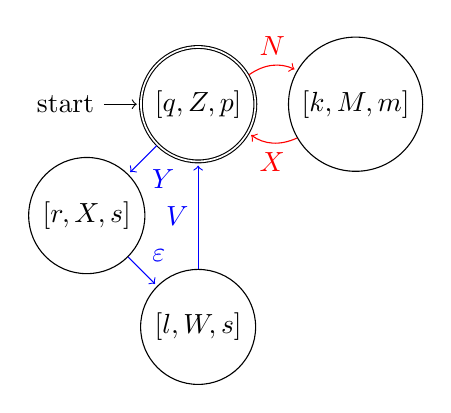
\begin{tikzpicture}[shorten >=1pt,node distance=2cm,on grid,auto] 
   \node[state,accepting] (i) [initial]  {$[q, Z, p]$}; 
     \node[state] (u) [below left=of i ]  {$[r, X, s]$}; 
  \node[state] (w) [below right=of u ]  {$[l, W, s]$}; 
     \node[state] (v) [right=of i]  {$[k, M, m]$}; 
    \path[->]          
    (i) edge [blue] node {$Y$} (u)
     (i) edge  [red, bend left, above] node {$N$} (v)
     (v) edge [red, bend left, below] node {$X$} (i)
    (u) edge [blue] node {$\varepsilon$} (w)
      (w) edge [blue]  node {$V$} (i);
\end{tikzpicture}
\\
	\caption{A possible computations of the PDA $M$ leading to the two different stack contents (left) and a corresponding part of NFA recognizing $L_{[q, Z, p]}$ (right).}
\label{densex}
\end{figure}
\begin{proof}
Consider an example of possible computation of a PDA $M$ in Figure~\ref{densex}. Without loss of generality suppose that $M$ has the following transitions from state $q$ to $q$, satisfying the criteria from the theorem:
\begin{itemize}
\item $\delta(q, \sigma, Z) \in (r, YX), (k, NM)$;
\item $\delta(r, \sigma', X) \in (l, W)$;
\item $\delta(l, \sigma'', W) \in (q, VZ)$;
\item $\delta(k, \sigma''', M) \in (q, XZ)$.
\end{itemize}
According to the construction of an NFA $\mathcal{A} = (S,\Gamma,\delta',[q_I, Z_0, q_f], t_f)$ recognizing pushdown store language of $M$ \cite{Malcher}, the NFA $\mathcal{A}$ has a state $[q, Z, p]$. Consider a new NFA $\mathcal{A}_{[q, Z, p]} = (S,\Gamma,\delta',[q, Z, p], \{[q, Z, p]\})$ with $L_{[q, Z, p]} = L(\mathcal{A}_{[q, Z, p]})$, which is illustrated in Figure~\ref{densex} (right). If there are at least two computations of PDA resulting in different stack contents for the same state $q$ and top symbol $Z$, where $[q, Z, p]$ is meaningful triple, then there are two paths $a$ and $b$ from $[q, Z, p]$ to $[q, Z, p]$ in NFA $\mathcal{A}_{[q, Z, p]}$ such that $ab \neq ba$. Thus, $L(\mathcal{A}_{[q, Z, p]})$ is not commutative and by Lemma~\ref{polyslender}, $P(M)$ has exponential density. If there is only variant of the stack contents, than NFA $\mathcal{A}_{[q, Z, p]}$ has only one path from $[q, Z, p]$ to $[q, Z, p]$ or several paths satisfying $ab = ba$ for each pair $a, b$ of these paths, therefore $L(\mathcal{A}_{[q, Z, p]})$ is commutative. If it holds for every meaningful triple, then $P(M)$ has polynomial density.
\end{proof}






\section{Closure properties of languages with polynomial rational indices}
\label{sec:closure}
Given a context-free language $L$ with a polynomial rational index, it is interesting to find which language operations preserve this property.  Boasson et al. \cite{RatBasic} give following useful relations for polynomial indices of two languages $L$ and $L'$.
\begin{theorem}[\cite{RatBasic}]
Context-free languages with polynomial rational indices are closed under intersection with a regular language, union, concatenation, homomorphism and inverse homomorphism. More precisely,
\begin{itemize}
\item $\rho_{L \cup L'} \le  \max{(\rho_L, \rho_{L'})} $
\item $\rho_{LL'} \le \rho_L + \rho_{L'}$
\item $\rho_{L \cap R}(n) \le \rho_L(nm)$, where $R$ is a regular language recognised by an $m$-state automaton
\item $\rho_{h(L)}(n) \le \rho_L(n)$ and $\rho_{h^{-1}(L)}(n) < n(\rho_L(n) +1)$, where $h: \Sigma^* \rightarrow \Delta^*$ is a homomorphism.
\end{itemize}
\end{theorem}
From the relations above it is easy to see that the family of context-free languages with polynomial rational indices is a full trio. Every full trio is closed under prefix and quotient with regular languages. Obviously, CFLs with polynomial rational indices languages are closed under reversal.  Next we show that context-free languages with polynomial rational indices are closed under Kleene star and insertion of a regular language (or context-free language with a polynomial rational index).
\begin{theorem}
Context-free languages with polynomial rational indices are closed under Kleene star and insertion of a regular language  (or context-free language with a polynomial rational index). Particularly,
\begin{itemize}
\item $\rho_{L^*}(n) \le n(\rho_L(n))$
\item $\rho_{LL'} \le \rho_L + \rho_{L'}$
\end{itemize}
\end{theorem}
\begin{proof}
\textit{Kleene star.} Let $G = (\Sigma, N, P, S)$ and $L(G)$ be a language with polynomial rational index. Consider language $L^{+}$, which grammar $G_1$ has the start nonterminal $S_1$. By definition of the Kleene plus operation, a rightmost derivation from $S_1$ generates a sequence of one or more start nonterminals $S$ from $G$, each of which generates some string in $L(G)$. Let $D$ be a directed labelled graph with $n$ nodes. Suppose there are nodes $u$ and $v$ in $D$ such that:
\begin{enumerate}
\item $v$ is not $L(G)$-reachable from $u$ and
\item $v$ is  $L^+$-reachable from $u$
\end{enumerate}
Then $v$ is reachable from $u$ via concatenation of words in $L(G)$. Consider the longest shortest path $u\pi_1 v$ between $u$ and $v$. It can be obtained by joining $(S, u, i), (S, i, j), ..., (S, w, v)$ into $(S_1, u, v)$.  If $L$ has the polynomial rational index, then for every realizable triple $(A, i, j)$ corresponding shortest path $i \pi j$ has at most polynomial length. There are no more than $O(n)$ such triples in concatenation because there are no repetitions of the same node in the sequence of start and end nodes of triples (otherwise $u\pi_1 v$ is not the shortest path, for example, path $u \rightarrow i \rightarrow k \rightarrow l \rightarrow i \rightarrow j \rightarrow v$ can be replaced with shorter path $u \rightarrow i  \rightarrow j \rightarrow v$), so $u\pi_1 v$ has at most polynomial length. In other words, we have $\rho_{L^+}(n) \le n(\rho_L(n))$.
\\
Family of languages with polynomial rational indices is a full trio closed under union, concatenation and Kleene star, therefore it is a full ALF. Full AFLs is known to be closed under substitution.
\\
\textit{Insertion of a regular language.} To prove closure under insertion of a regular language, the following PDA can be constructed. Let $L$ be a context-free language with polynomial rational index and let $M$ be a PDA recognizing $L$. New PDA $M'$ for insertion of a regular language $R$ recognized by finite automation $F$ into $L$ can be obtained as follows: duplicate all states in $M$, initial state is placed in first set and final states reside in the second set. Every state in the first set has its own copy of outgoing arcs of the initial state of $F$. Every ingoing arc of final state of $F$ is connected directly to every state of the second set of $M$. In other words, every state from the first set is the initial state of $F$ and every state from the second set is a final state of $F$. All arcs from $F$ are labelled the same way as they are labelled in $F$.
Consider intersection of $M'$ and arbitrary finite automotion $F'$ with $n$ states. The longest non-empty shortest path $i \pi j$ in the intersection of $M'$ and $F'$ consists of three sub-paths: $i\pi_1k$, $k\pi_2m$ and $m\pi_3j$, where $i\pi_1k$ ($m\pi_3j$) is the shortest paths in the intersection of $F'$ and first (second) set of states of $M$ respectively, and $k\pi_2m$ is the shortest path in the intersection of $F'$ and $F$. $k\pi_2m$ has at most polynomial length because all regular languges have polynomial rational indices, $i\pi_1k$ and $m\pi_3j$ have polynomial length because $M$ is a PDA for language with rational index, therefore  $i \pi j$ has polynomial length.
\end{proof}


Using closure properties, it is easier to find new subclasses of context-free languages for which CFL-reachability problem is in NC.
\begin{example}[Metalinear languages \cite{metalinear}.]
\\
Let $G = (\Sigma, N, P, S)$ be a context-free grammar. $G$ is \textit{metalinear} if all productions of $P$ are of the following forms:
\begin{enumerate}
\item $S \rightarrow A_1A_2...A_k$, where $A_i \in N - \{S\}$
\item $A \rightarrow u$, where $A \in N \setminus \{S\}$ and $u \in (\Sigma^*((N \setminus \{S\}) \cup {\varepsilon})\Sigma^*)$
\end{enumerate}


The width of a metalinear grammar is $max\{k$ | $S \rightarrow A_1A_2...A_k \}$. Metalinear languages of width 1 are obviously linear languages. It is easy to see that every metalinear language is a union of concatenations of $k$ linear languages. Linear languages have polynomial rational index,  CFLs with polynomial rational index are closed under concatenation and union, so metalinear languages have polynomial rational index.
\end{example}


\section{Conclusions and open problems}
\label{sec:conc}
\begin{figure}
\centering
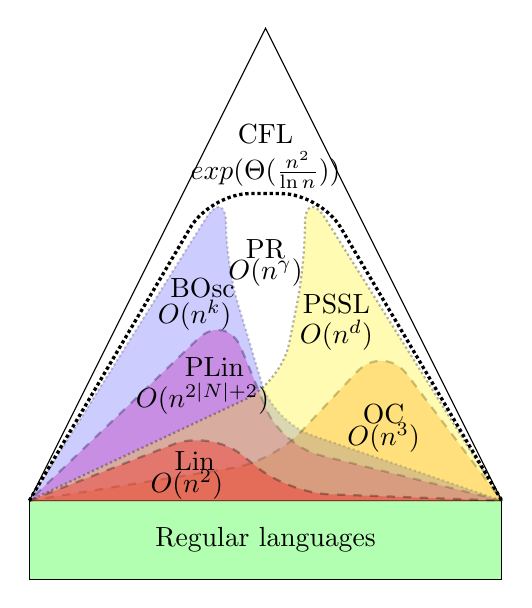
\begin{tikzpicture}
\draw[fill=green, opacity=0.3](0,1) -- (0,0) -- (6,0) --  (6,1);
\draw(0,1) -- (0,0) -- (6,0) --  (6,1);
\draw(0,1) -- (6,1) -- (3, 7) -- (0,1) ;
\draw[thick, dashed, rounded corners=5mm, fill=orange, opacity=0.3] (0,1) -- (3.1, 1.5) -- (4.5, 3) -- (6,1);
\draw[thick, dashed, rounded corners=5mm, fill=magenta, opacity=0.3] (6,1) -- (3.2, 1.7) -- (2.5, 3.4) -- (0,1);
\draw[thick, densely dotted, rounded corners=5mm, fill=blue, opacity=0.2](0,1) -- (2.5, 5) -- (2.5,4)-- (3.1, 2) -- (6,1);
\draw[thick, densely dotted, rounded corners=5mm , fill=yellow, opacity=0.3](6,1) -- (3.5, 5) -- (3.5,4)-- (3.2, 2.5) -- (0,1);
\draw[thick, dashed, rounded corners=5mm, fill=red, opacity=0.3] (0,1) -- (2.3, 1.9)  -- (3.3, 1.1) -- (6,1);
\draw[very thick, densely dotted, rounded corners=5mm] (0,1) -- (2.3, 4.9) -- (3.7, 4.9) -- (6,1);
\node (reg) at (3, 0.5) {Regular languages}; 
\node (cfl) at (3, 5.65) {CFL}; 
\node (pr) at (3, 4.2) {PR};
\node (prrho) at (3, 3.9) {$O(n^\gamma)$};
\node (cflrho) at (3, 5.2) {$exp(\Theta(\frac{n^2}{\ln n}))$}; 
\node (plin) at (2.35, 2.7) {PLin}; 
\node (lin) at (2.1, 1.5) {Lin}; 
\node (osc) at (2.2, 3.7) {BOsc}; 
\node (one) at (4.5, 1.8) {$O(n^3)$}; 
\node (onerho) at (4.5, 2.1) {OC}; 
\node (pssl) at (3.9,3.5) {PSSL}; 
\node (psslrho) at (3.9,3.1) {$O(n^{d})$}; 
\node (linrho) at (2, 1.2) {$O(n^2)$}; 
\node (linrho) at (2.2, 2.29) {$O(n^{2|N|+2})$}; 
\node (oscrho) at (2.1, 3.35) {$O(n^{k})$}; 
\end{tikzpicture}
\caption{The hierarchy of languages with polynomial rational indices and corresponding upper bounds on the value of rational index. PR --- the family of CFLs with a polynomial rational indices, BOsc --- bounded-oscillation languages, PSSL --- CFLs with poly-slender storage languages, PLin --- piecewise linear languages, OC --- one-counter languages, Lin --- linear languages, $n$ --- number of vertices in graph (NFA), $|N|$ --- the number of non-terminals of grammar in Chomsky normal form, $k$ --- the oscillation value, $d$ --- degree of polynomial density of a pushdown storage language, $\gamma$ --- algrebraic number.}
\label{hierarchyfinal}      
\end{figure}
We have obtained two classes, which extend the classes in the recent literature \cite*{ChainQ, LabelledGraphs, LReach, Regularrealizability, Ullman}, for which CFL-reachability problem is in NC. The one is the class of bounded-oscillation languages, which generalizes the linear languages. The second class is context-free languages with a poly-slender pushdown store languages, which is generalization of the one-counter languages. Recall that regular languages have polynomial fringe property (and are accepted by PDA with a bounded stack height), also it is known that L-reachibility for regular languages is in NL \cite*{LReach, Yannakakis}. Thereby it has been demonstrated that some natural restrictions on the pushdown storage implies polynomial rational index for the corresponding context-free languages: low variability of stack height during the PDA run (bounded-oscillation PDA) and limited number of possible stack contents (languages with poly-slender pushdown store languages). The updated hierarchy of tractable subclasses and corresponding upper bounds on the rational indices are illustrated in Figure~\ref{hierarchyfinal}.


It will be interesting to know whether there is another kind of stack restriction which implies polynomial rational index. Or is there a context-free language which does not belong to any of the above mentioned classes? Are there any other properties (except polynomial rational index) which make the CFL-reachability problem solvable in NC? For example there is a Datalog query, which does not have a polynomial fringe property but its evaluation is in NC \cite{Kanellakis}. One can also approach this question from another direction by looking for simple subfamilies of context-free languages that would have P-complete CFL-reachability problem.

We considered CFL-reachability problem for a fixed context-free languages and arbitrary graphs. What tractable cases can be obtained for a fixed graphs and an arbitrary context-free language? The known and trivial examples are acyclic graphs and trees. Can we have more complicated classes of graphs for which CFL-problem is in NC? Interesting algebraic properties of such graphs (NFA) are given in \cite{ganardi2016circuit}, but automata-theoretic characterizations of these properties remain to be found.
\bibliographystyle{spbasic}      % basic style, author-year citations
\bibliography{paper}   % name your BibTeX data base
\end{document}
% end of file template.tex